\documentclass[12pt]{article}
\author{Lawrence Liu, UID: 405749034}
\usepackage{subcaption}
\usepackage{graphicx}
\usepackage{amsmath}
\usepackage{pdfpages}
\newcommand{\Laplace}{\mathscr{L}}
\setlength{\parskip}{\baselineskip}%
\setlength{\parindent}{0pt}%
\usepackage{xcolor}
\usepackage{listings}
\definecolor{backcolour}{rgb}{0.95,0.95,0.92}
\usepackage{amssymb}
\usepackage{empheq}

\newcommand*\widefbox[1]{\fbox{\hspace{2em}#1\hspace{2em}}}
\lstdefinestyle{mystyle}{
    backgroundcolor=\color{backcolour}}
\lstset{style=mystyle}
\title{Chem 20A Worksheet 3}
\begin{document}
\maketitle
\section*{Problem 1}
We have that the 4d orbitals have 1 radial node and 2 angualr nodes, the possible quantum states are:
(4,2,-2),(4,2,-1),(4,2,0),(4,2,1),(4,2,2). For the 5f orbitals, the possible quantum states are
(5,3,-3),(5,3,-2),(5,3,-1),(5,3,0),(5,3,1),(5,3,2),(5,3,3). The 5f Orbitals have 1 angular and 3 radial 
nodes.
\section*{Problem 2}
\subsection*{(a)}
We have that the 5dxy orbital has 2 radial nodes, and 2 angular node planes, one along the xz 
plane and one along the zy plane. See the figure below for the sketch of the 5dxy orbital.\\
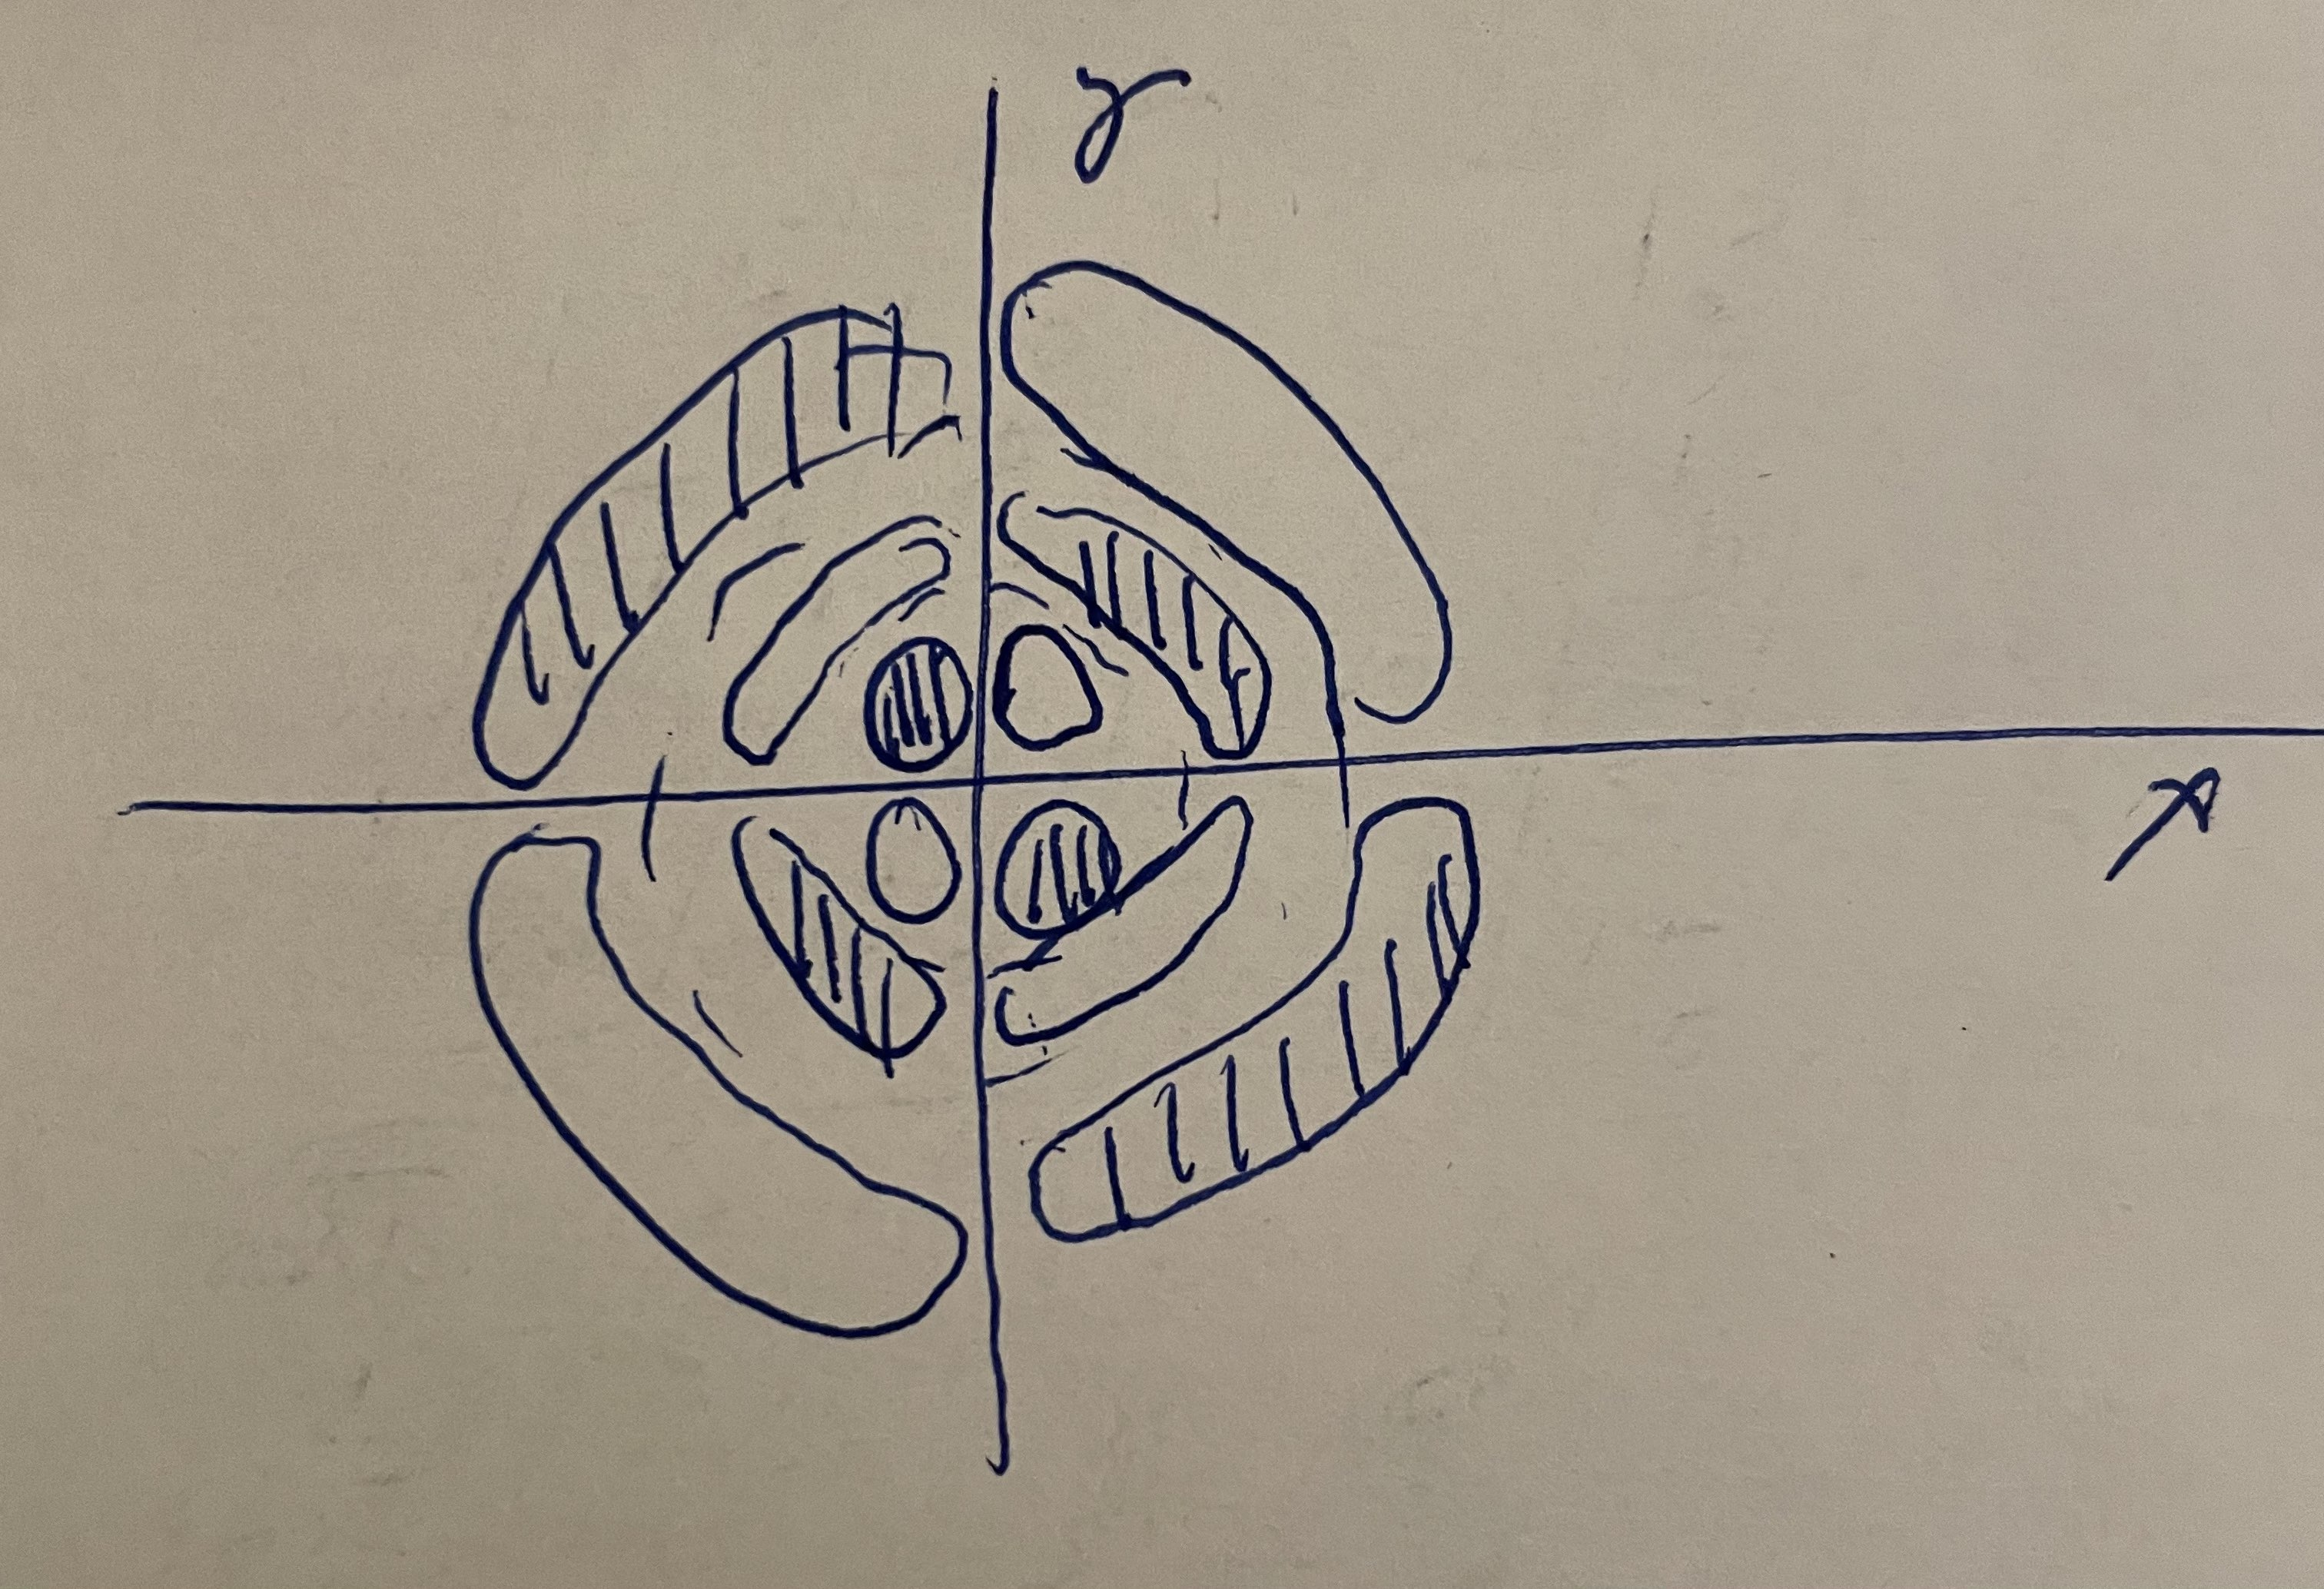
\includegraphics[width=0.5\textwidth]{5dxy.png}
\\
We have that the angular nodes occur when 
$$40-14\sigma+\sigma^2=0$$
We have that this occurs where $\sigma=4$ and $\sigma=10$. Since 
$\sigma=\frac{2Zr}{na_0}$, we have that the corresponding radiuses from the origin is
$$r=\frac{na_0\sigma}{2Z}$$
Thus we have that the radiuses from the origin where the angular nodes occur are
$r=\boxed{13.229\AA}$ and $\boxed{5.291\AA}$.
\subsection*{(b)}
We have that the average readius is given by
$$r=\frac{5^2a_0}{Z}\left(1+\frac{1}{2}\left(1-\frac{6}{25}\right)\right)=\boxed{18.256\AA}$$
\section*{Problem 3}
\subsection*{(a)}
We have that the radial probability function is given by 
$$P(r)=4r^2\left(\frac{1}{a_0}\right)e^{-\frac{2r}{a_0}}dr$$
Therefore 
$$P(a_0)=\frac{4}{a_0}e^{-2}\cdot 10^{-3}a_0=4e^{-2}\cdot 10^{-3}=0.000541$$
\subsection*{(b)}
We have that
$$P(1)=0$$
\end{document}
